\documentclass{article}
\usepackage[utf8]{inputenc}
\usepackage[portuguese]{babel}
\usepackage[a4paper, total={7in, 9in}]{geometry}
\usepackage{graphicx}
\usepackage{float}
\usepackage[title]{appendix}
\usepackage[style=numeric]{biblatex}
\usepackage{csquotes}
\usepackage{mathtools}
\addbibresource{references.bib}

\begin{document}

{
\center
\textsc{\Large Universidade do Minho} \\ [0.5cm]
\textsc{\Large Mestrado em Engenharia Informática} \\ [0.5cm]
\textsc{\large Paradigmas de Computação Paralela} \\ [0.5cm]

{\LARGE \bfseries Paralelização de um algoritmo de simulação de ondas sonoras através de códigos stencil} \\[0.5cm]

\begin{tabular}{c c}
    José Carlos Lima Martins & Miguel Miranda Quaresma \\
    A78821 & A77049  \\
\end{tabular} \\[0.5cm]

\today \\[1cm]
}

\section{Introdução}
O desenvolvimento de aplicações paralelas compreende dois grandes paradigmas 
que diferem na forma como a memória é gerida \textbf{i.e.} se esta é partilhada (OpenMP) ou
distribuída (MPI). Como tal, no seguimento da implementação de um algoritmo \textit{stencil}
num paradigma de memória partilhada, o presente trabalho propõe-se a realizar esta 
implementação num paradigma de memória distribuída com MPI (Message Passing Interface).

Numa primeira fase, na secção \ref{desenho}, será descrita a abordagem elaborada para 
implementar este algoritmo no paradigma de memória distribuída com processos comunicantes. 
De seguida, na secção \ref{analise}, será feita uma análise teórica ao algoritmo de forma a 
determinar, previamente, a escalabilidade do mesmo. Com o intuito de melhorar a compreensão dos
resultados apresentados na secção \ref{comp}, na secção \ref{context} é apresentada uma descrição
do contexto em que os testes foram realizados. A apresentação e discussão dos resultados 
experimentais, realizada na secção \ref{comp}, compreenderá o estabelecimento de comparações 
entre os tempos sequenciais e os paralelos e justificação dos resultados observados. 
Por fim, na secção \ref{concl}, são apresentadas as conclusões relativamente ao comportamento 
deste tipo de algoritmos (\textit{stencil}) num paradigma de memória partilhada.

\section{Desenho da implementação MPI} \label{desenho}
Os algoritmos de simulação de ondas sonoras envolvem o uso de padrões \textit{stencil} na sua implementação. Na 
aplicação desenvolvida o \textit{stencil} utilizado possui uma vizinhança de tamanho 4 em cada direção(horizantal, vertical) e sentido(positivo, negativo) e envolve a atualização de todos os pontos que não pertençam às 4 primeiras 
e 4 últimas linhas/colunas. A cada iteração do algoritmo(\textit{stencil}) cada ponto toma o valor correspondente 
à soma dos 17 pontos na sua vizinhança, incluindo o próprio ponto, filtrados por uma máscara que é aplicada com base na
distância de cada ponto ao centro da vizinhança.

Por forma a paralelizar este algoritmo num paradigma de memória distribuída com base no MPI, torna-se necessário distribuir a carga pelos 
diferentes processos. Esta função é da responsabilidade do processo com \textit{rank} 0, que distribui as linhas da 
matriz (de tamanho M\_SIZE) por P processos, delegando a cada processo $\frac{M\_SIZE-8}{P}$ linhas mais 8 linhas (4 
linhas imediatamente abaixo e acima da secção atribuída) que permitam o cálculo dos valores sem que haja comunicação 
entre processos, dentro de cada iteração. Por forma a dividir a carga, realiza-se uma divisão inteira entre a carga a 
distribuir (sem as 4 primeiras e últimas linhas) e o número de processos (P). Caso o número de linhas não seja
múltiplo do número de processos, as restantes linhas são distribuídas, de forma iterativa, pelos processos, começando
pelo processo com \textit{rank} 1. Com esta forma de distribuição é possível garantir que a diferença de carga entre processos não excede uma linha. Esta divisão pode ser visualizada no anexo \ref{divMatrix}. 

Depois da distribuição da matriz, serão realizadas \textit{it} iterações em que cada processo atualizará os pontos 
das linhas que lhe foram atribuídas. Ao fim de cada iteração, cada processo troca, com os processos adjacentes
(rank-1, rank+1), as linhas com os valores atualizados que permitam aos processos iniciar a iteração seguinte. Após 
a realização de todas as iterações, todos os processos enviam os resultados para o processo com o \textit{rank} 0, 
que armazena estes valores na matriz original. Por forma a facilitar a implementação e compreensão deste mecanismo foi 
desenvolvido o modelo presente no anexo \ref{procsMPI}. 

Por fim é importante referir que o número de processos P compreende apenas os processos que participam na 
atualização dos valores da matriz, não incluindo o processo com \textit{rank} 0. Como consequência, para que 
sejam usados P processos na computação do \textit{stencil} são necessários P+1 processos.

\section{Análise teórica do algoritmo} \label{analise}
A implementação de algoritmos em paradigmas de memória distribuída em que existe 
comunicação inter-processos beneficia da elaboração de modelos teóricos que permitam
avaliar, sem a realização de testes, se um dado algoritmo escala face ao número de 
processos. Para isso é importante ter em conta as diversas fases que compõem uma 
implementação MPI e o tempo que cada uma ocupa: 
\begin{enumerate}
    \item Fase de computação: $T_{comp}$
    \item Fase de comunicação: $T_{comm}$
    \item Tempo \textit{idle}(livre): $T_{free}$
\end{enumerate}
Estes valores permitem obter uma aproximação do tempo de execução através da seguinte 
expressão: \label{t_par}
$$T_{exec} = T_{comp} + T_{comm} + T_{free}$$

\subsection{Computação: $T_{comp}$}
A fase de computação do algoritmo de \textit{stencil} compreende o cálculo, a cada
iteração, do valor de cada ponto com base nos pontos da sua vizinhança. Como tal, a 
expressão usada no tempo de computação deve ser a seguinte:
$$it * ops\_per\_element * elements\_per\_process * tc$$
onde $tc$ corresponde ao tempo por operação aritmética e $it$ corresponde ao número
de iterações realizadas pelo algoritmo. O valor $tc$ foi calculado através de uma benchmark 
(\ref{pingpong_mpi} - função computation\_test) sendo o seu valor igual a $tc=0.00141907 us/op$. 
No caso de um algoritmo \textit{stencil} que apresente a seguinte fórmula geral:
\begin{verbatim}
    G[i][j] = C[0]*G[i][j] + 
              ... 
              C[N]*G[i][j+N] + 
              C[N]*G[i+N][j];
\end{verbatim}
o número de operações por elemento varia de acordo com o tamanho da vizinhança, 
correspondendo ao número de somas e multiplicações efetuadas. Num \textit{stencil} 
de 17 pontos são efetuadas 16 adições e 17 multiplicações, totalizando 33 operações 
aritméticas por elemento. Considerando uma matriz de tamanho $M\_SIZE$ e $P$ processos, 
o número de elementos a processar por linha será $M=M\_SIZE-8$, dado que os 4 primeiros 
e últimos pontos de cada linha não são considerados no cálculo. Substituindo os valores 
correspondentes na fórmula indicada obtém-se:
$$T_{comp} = it*\frac{33*M^2}{P}*tc$$

\subsection{Comunicação: $T_{comm}$}
Num paradigma de memória distribuída com processos comunicantes
o maior limitador de \textit{performance} é a comunicação entre processos, como tal esta 
fase será fulcral na determinação da escalabilidade de um dado algoritmo: quanto menor for o seu peso no tempo de execução, maior será a escalabilidade do algoritmo. Este tempo pode ser calculado tendo em conta a latência da comunicação($ts$) bem como a largura de banda($1/tw$) da comunicação: 
$$ T_{comm} = messages\_per\_proc * (ts + tw*L) $$ 
em que $L$ corresponde ao tamanho(em \textit{bytes}) do input a transmitir.
Os parâmetros $ts$ e $tw$ podem ser obtidos através da realização de uma \textit{benchmark Ping-Pong}, que consiste em trocar mensagens entre dois processos e medir o tempo de 
transmissão das mesmas, variando o tamanho da mensagem consoante se pretenda determinar a 
latência ou a largura de banda do sistema em questão.
Para este efeito foi desenvolvida uma \textit{benchmark} (\ref{pingpong_mpi}) através da 
qual se obtiveram os seguintes valores:
\begin{itemize}
    \item $ts=122.5104054 us$
    \item $tw=0.08621396 us$
\end{itemize}

Dado $L$ corresponder ao tamanho do input a transmitir, este será dado por $L=4*M\_SIZE*8$, 
onde 4 corresponde ao tamanho do \textit{stencil} e 8 ao tamanho, em \textit{bytes}, de 
um \texttt{double}. Substituindo os valores referidos, obtém-se, para a troca de linhas
entre processos:
$$T_{inter\_proc} = it*2*(ts+4*8*M\_SIZE*tw)$$
Mais uma vez, esta fase toma lugar todas as iterações, algo representado pelo produto
por $it$.

Para além da comunicação inter-processo a presente implementação compreende uma fase de 
distribuição de dados pelos processos e uma fase de recolha de resultados. Como tal, esta 
fase é formulada da seguinte maneira:
$$T_{dist} = 2*((M\_SIZE*M+M\_SIZE*4*P)*tw+ts*P)$$

Finalmente para obter $Tcomm$ basta somar os dois tempos referidos anteriormente [ver \ref{formulas}-\ref{eq:Tcomm}]:
$$T_{comm} = T_{inter\_proc} + T_{dist}$$


\subsection{Idle: $T_{free}$}
O tempo em que determinados processos se encontram \textit{idle} é muitas vezes motivado 
pela má distribuição da carga entre os diversos processos. No entanto, na implementação 
descrita, a carga encontra-se uniformemente distribuída entre os diversos processos
havendo, no máximo, uma linha adicional para determinados processos(em casos em que o 
número de elementos não é múltiplo do número de processos). Como tal, para a presente análise 
este valor será considerado nulo: 
$T_{free} \approx 0$.

\subsection{Escalabilidade/Speed-Up}
A análise teórica do algoritmo exige o recurso a uma métrica que seja mais relevante do
que o seu tempo de execução. Como tal,o \textit{speed-up} \textbf{i.e}
redução no tempo de execução face ao aumento no número de processos, é a métrica usada
nesta análise.

\subsubsection{Tempo Paralelo}
Como foi referido anteriormente (\ref{t_par}), o tempo de execução paralelo, para um 
dado número de processos \textbf{P}, pode ser expressado através da seguinte fórmula [ver \ref{formulas}-\ref{eq:Tpar}]:
$$T_{par} = T_{comp} + T_{inter\_proc} + T_{dist}$$

\subsubsection{Tempo Sequencial}
O tempo sequencial do algoritmo \textit{stencil} poderá ser aproximado pela fórmula
$T_{seq}=T_{comp}*P$ dado que, neste paradigma, não existe comunicação entre processos o tempo de comunicação é nulo ($T_{comm}=0$).
O tempo de execução sequencial será: 
$$T_{seq} = T_{comp}*P = it*33*M^2*tc$$

\subsubsection{Speed-Up}
O \textit{speed-up}(G) corresponde à razão entre o tempo paralelo e o (melhor) tempo sequencial,
sendo dado pela seguinte expressão [ver \ref{formulas}-\ref{eq:G}]:

$$G=\frac{T_{seq}}{T_{par}} = \frac{P*T_{comp}}{T_{comp} + T_{inter\_proc} + T_{dist}}$$

Aplicando a fórmula às diversas configurações (tamanho da matriz (M\_SIZE) e número de iterações
(it)) usadas nos testes permite prever a escalabilidade do algoritmo, como é possível observar
no gráfico \ref{theoretical_g}.

\section{Contexto de experimentação e testes realizados} \label{context}
\subsection{Hardware utilizado}
Os testes de seguida descritos foram realizados em nodos r641 do \textit{cluster} SeARCH que apresentam
a seguinte configuração (de hardware):
\begin{itemize}
    \item \textbf{CPU}: 2 * Intel Xeon E5-2650v2
        \begin{itemize}
            \item \textbf{Frequência}: 2.6GHz
            \item \textbf{Nro. de Cores}: 8 físicos, 16 lógicos com \textit{Hyper-threading}
            \item \textbf{Cache L2}: 256 KB por core físico
            \item \textbf{Cache L3}: 20MB por socket
        \end{itemize} 
    \item \textbf{Memória RAM}: 64 GB
\end{itemize}

O código (fonte) foi compilado com a versão 5.3.0 do compilador GCC e a versão 2.0.0 da biblioteca OpenMPI-Ethernet.

\subsection{Parâmetros experimentais}
Os testes foram realizados alterando os seguintes parâmetros:
\begin{itemize}
    \item \textbf{M\_SIZE ordem da matriz}: 128, 895, 2100
    \item \textbf{IT número de iterações}: 64, 256, 1024
    \item \textbf{Número de processos utilizados}: 2, 4, 8, 16, 32, 64
    \item \textbf{Mapeamento de processos (\texttt{--map-by})}: \texttt{core, node, slot}
    \item \textbf{Número de nodos r641 utilizados}: 1, 2
\end{itemize}
Os valores para o tamanho da matriz(M\_SIZE) foram escolhidos por forma a explorar os diferentes níveis da hierarquia 
de memória [cálculos presentes em \ref{calOrdem}]:
\begin{itemize}
    \item 128x128: que cabe na cache L2
    \item 895x895: que cabe na cache L3
    \item 2100x2100: que apenas cabe na memória principal
\end{itemize} 
O valores escolhidos para o número de iterações crescem exponencialmente (64, 256, 1024), sendo diretamente proporcionais ao tamanho da matriz.

A biblioteca OpenMPI permite que a forma como os processos são mapeados nas unidades de processamento 
disponíveis seja alterada ``\textit{at runtime}''. Como tal os testes realizados exploram diferentes
mapeamentos para identificar possíveis ganhos:
\begin{itemize}
    \item \texttt{--map-by core} : distribuição dos processos por cada core físico, colocando mais que um processo por core apenas quando todos(os cores) 
    estiverem ocupados, aproveitando o \textit{Hyper-Threading}
    \item \texttt{--map-by node} : distribuição dos processos por nodos, de forma cíclica (round-robin), resultando numa distribuição uniforme dos
    processos
    \item \texttt{--map-by slot} : distribuição dos processos por \textit{slots}, semelhante ao \texttt{--map-by core}, em que cada core é visto como dois
    \textit{slots} consecutivos devido ao \textit{Hyper-Threading}
\end{itemize}

\subsection{Testes realizados}
Os parâmetros anteriormente descritos foram combinados por forma a contemplar diversos cenários
permitindo obter uma análise mais compreensiva do comportamento da aplicação desenvolvida no
presente paradigma. As configurações utilizadas encontram-se presentes na tabela \ref{lab_config}.

É importante salientar que, para a configuração M\_SIZE=128 e IT=64, não foram realizados testes para 
um número de processos igual a 32 e a 64 dado que, nestes casos, o número de linhas por processo seria 
inferior a 4, que é o tamanho da vizinhança do \textit{stencil}. Esta distribuição apresentaria duas consequências
negativas:
\begin{itemize}
    \item ineficiência causada pelo facto de que, para cada processo, a quantidade de dados trocados seria superior à quantidade de dados processados
    \item implementação mais complexa que levaria a um decréscimo da \textit{performance} ao exigir o recurso a estruturas condicionais que permitissem 
    impedir a transmissão de dados redundantes
\end{itemize}

\subsection{Testes adicionais}
Para além dos testes anteriormente referidos foram ainda realizados testes que permitissem, para cada uma das 
configurações indicadas, determinar a fração de tempo que correspondia a comunicação inter-processos.

\subsection{Metodologia de experimentação}
Por forma a obter valores normalizados, precisos, reproduzíveis e limitar a influência de \textit{outliers} nos valores considerados foram
recolhidas, para cada teste, 15 amostras e o valor da mediana tomado como o tempo de execução para a configuração 
correspondente.

\section{Análise de resultados experimentais} \label{comp}
Após a análise teórica, foram realizados testes que permitissem obter tempos de execução para a aplicação 
desenvolvida. 

\subsection{Análise teórica vs. Dados Experimentais}
Uma análise dos dados experimentais recolhidos (\ref{speedup_tbl}) e do gráfico de escalabilidade resultante
(\ref{mpi_speedup_graph}) permite identificar uma tendência anteriormente observada na análise teórica: a 
escalabilidade da aplicação para um número de processos superior a 16 é reduzida, sendo ainda possível observar um decréscimo no 
ganho obtido quando o número de processos ultrapassa este valor(16). Uma inspeção mais detalhada das diferentes fases 
do algoritmo, e da fase de comunicação em específico, permite identificar a causa deste decréscimo no ganho de 
performance: para execuções em que o número de processos é superior a 16, a latência associada à comunicação 
inter-processos anula o benefício conseguido na paralelização da aplicação. \label{mpi_loss_scalability}
Por outro lado, o \textit{speed-up} previsto pela análise teórica serve de teto ao \textit{speed-up} observado, 
algo que seria expectável dado o facto deste tipo de análise(teórica) não considerar fatores como escalonamento
de processos no processador ou acessos não uniformes à memória (NUMA). 

É importante observar o comportamento da implementação no caso em que são usados 2 processos (P+1) visto que 
este ilustra o impacto que a comunicação tem no desempenho da aplicação: a perda de \textit{performance} é causada
pelo facto de que apenas um dos dois processos efetua os cálculos, resultando numa execução sequencial à qual acresce
a fase de comunicação inicial/final entre os dois processos, levando à perda de \textit{performance}.

Para além disso é possível perceber que, quando a matriz é de reduzidas dimensões, o ganho na paralelização por MPI
(e OpenMP) é reduzido devido à pequena quantidade de dados a calcular.

Já entre um e dois nodos, verifica-se que com mais de 16 cores, a escalabilidade num nodo é menor em relação à observada em dois 
nodos pelo simples facto de que, no caso em que dois nodos são utilizados, os processos são escalonados sem que seja
necessário escalonar mais que um processo por \textit{core} lógico, permitindo a capacidade de \textit{Hyper-threading}.

Por fim, denota-se que com um nodo não há grande distinção entre mapeamento \texttt{by core}, \texttt{by node} e \texttt{by slot}, 
visto que a distribuição efetuada é semelhante em consequência do uso de um único nodo.
Pelo contrário, com dois nodos, como no caso anterior, o comportamento apresentado pelos mapeamentos \texttt{by core} e \texttt{by node} é semelhante, enquanto que o mapeamento \texttt{by node} apresenta pior \textit{performance} causada pela comunicação entre processos por \textit{Ethernet}.


\subsection{Comparação entre paradigmas de aplicações paralelas}
Um dos aspetos mais importantes no desenvolvimento de aplicações paralelas é a identificação do paradigma que mais
se adequa a um dado \textit{use-case}, se um paradigma de memória partilhada se um de memória distribuída.
Nesse sentido torna-se relevante comparar a versão OpenMP deste algoritmo \textit{stencil} com a versão
OpenMPI.

A observação dos gráficos de \textit{speed-up} para cada um dos casos(\ref{mp_speedup_graph} e 
\ref{mpi_speedup_graph}) permite tirar conclusões quanto à escalabilidade dos mesmos. Apesar de ambas as
implementações apresentarem, de forma geral, ganho face à versão sequencial até um número de \textit{threads}/processos 
igual a 16, um dos aspetos mais evidentes é o facto do paradigma de memória partilhada (OpenMP) apresentar uma 
escalabilidade que se aproxima da ideal até um número de \textit{threads} igual a 16 (inclusive), algo que não 
se verifica na implementação MPI. Como foi referido anteriormente (\ref{mpi_loss_scalability}), um dos fatores
que limitam a versão MPI para um número de processos superior a 16 é a comunicação existente entre esses mesmos
processos, algo que não tem lugar numa versão OpenMP, em que esta comunicação é substituída pelo uso de regiões 
de memória partilhada. 


\subsection{Perfil de Execução}
Com o intuito de melhorar a compreensão dos diferentes fatores que influenciam o comportamento verificado para 
cada uma das versões referidas torna-se indispensável traçar um perfil de execução para as mesmas. Este perfil
consiste em discriminar o peso de cada um dos componentes que constituem o tempo de execução (sec. \ref{t_par}) no 
valor do mesmo. Com este intuito foram realizados testes que permitiram identificar que percentagem do tempo de 
execução é ocupada pela comunicação entre processos. Os resultados presentes no histograma \ref{comm_time_perc}, 
indicam um tendência clara (e previsível): quanto maior o número de processos, maior será a influência do tempo de 
comunicação no tempo de execução. Este comportamento é justificado pelo facto de que, apesar da carga por
processo diminuir com o número de processos e consequentemente, o tempo de computação ($T_{comp}$), o número
de mensagens trocadas entre processos aumenta (\ref{data_flux}).
O perfil de execução em conjunção com a escalabilidade observada permite identificar a clara influência que 
a fração de código correspondente à comunicação tem na escalabilidade da aplicação, sendo esta (comunicação) a maior 
limitadora de \textit{performance} visto que a margem para melhoramento é nula dado a comunicação entre dois
processos ser algo inerentemente sequencial. É importante referir que este comportamento seria o esperado se
for tida em conta a lei de Amdahl \cite{amdahl_multicore}.

\section{Conclusão} \label{concl}
A análise dos resultados realizada, bem como as diversas comparações permite identificar um limitador
comum de performance em todos os casos: comunicação inter-processo. Consequentemente, torna-se imperativo 
o recurso a técnicas que permitam reduzir a frequência destas comunicação, nomeadamente o recurso a informação 
redundante. 
Adicionalmente, o desenvolvimento de aplicações num paradigma de memória distribuída em MPI apresenta diversas
desvantagens que levam a que implementações com recurso a OpenMP sejam preferidas, nomeadamente a complexidade
acrescida do código face à escalabilidade observada.

\printbibliography

%\onecolumn

\begin{appendices}

\section{Divisão da matriz}
\label{divMatrix}
\begin{figure}[H]
    \centering
    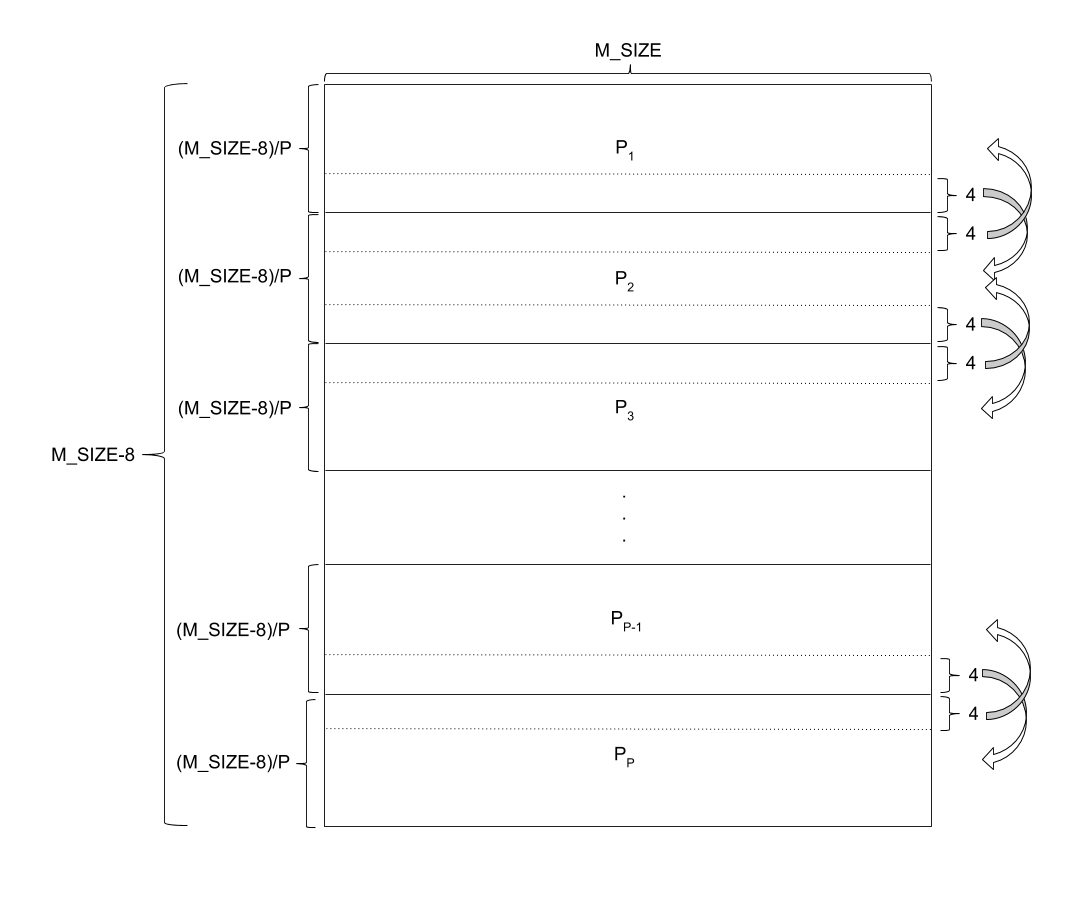
\includegraphics[width=15cm]{Pictures/matrixDraw.png}
\end{figure}


\section{Papel dos processos}
\label{procsMPI}
\begin{figure}[H]
    \centering
    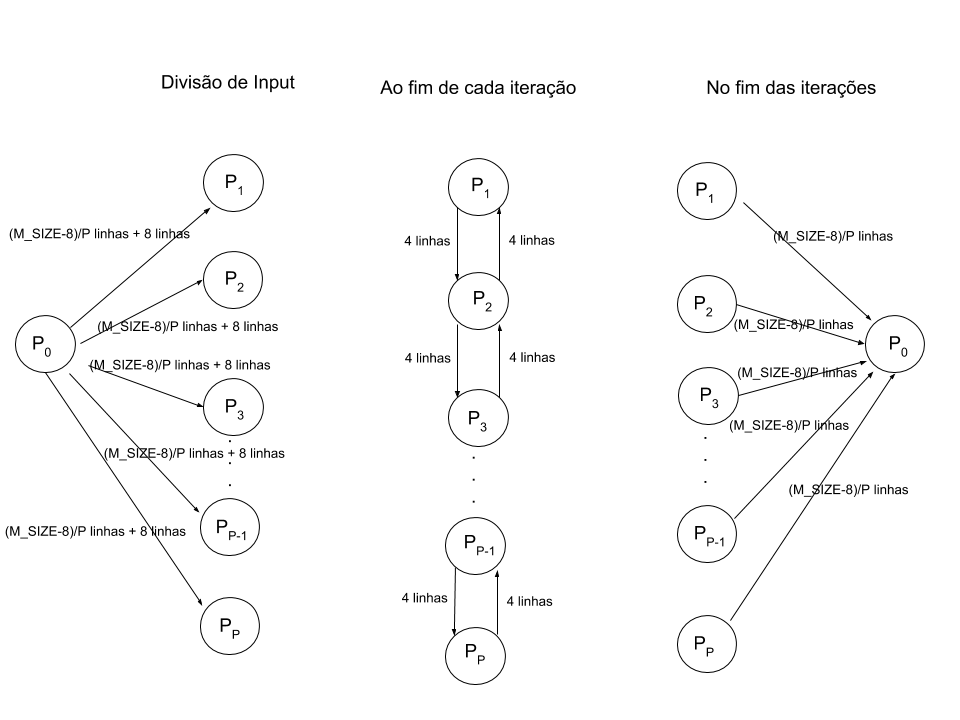
\includegraphics[width=15cm]{Pictures/graphDraw.png}
\end{figure}


\section{Análise Teórica-Fórmulas} \label{formulas}
\begin{equation}
T_{comp} = it*\frac{33*M^2}{P}*tc \label{eq:Tcomp}
\end{equation}

\begin{equation}
T_{comm} = 2*((M\_SIZE*M+M\_SIZE*4*P)*tw+ts*P) +  it*2*(ts+4*8*M\_SIZE*tw) \label{eq:Tcomm}
\end{equation}

\begin{equation}
T_{par} = it*\frac{33*M^2}{P}*tc + 2*((M\_SIZE*M+M\_SIZE*4*P)*tw+ts*P) +  it*2*(ts+4*8*M\_SIZE*tw) \label{eq:Tpar}
\end{equation}

\begin{equation}
T_{seq} = it*33*M^2*tc \label{eq:Tseq}
\end{equation}

\begin{equation}
G=\frac{it*33*M^2*tc}{it*\frac{33*M^2}{P}*tc + 2*((M\_SIZE*M+M\_SIZE*4*P)*tw+ts*P) + it*2*(ts+4*8*M\_SIZE*tw)} \label{eq:G}
\end{equation}

\section{Cálculo da Ordem das Matrizes} \label{calOrdem}
\begin{itemize}
    \item 128x128: que cabe na cache L2 \newline
          O pior caso será caso a matriz não seja dividida, ou seja P=1: \newline
          $ (x * x)* 2 = \frac{256*1024}{8} \Leftrightarrow x = 128 $ \newline
          \begin{equation}
              \begin{split}
                   ordem\_matriz * matrizes\_por\_processo = \frac{tamanho\_da\_cache(bytes)}{tamanho\_de\_um\_double(bytes)}
              \end{split}
          \end{equation}

    \item 895x895: que cabe na cache L3 \newline
          $ x*x + (15*(\frac{x}{15} + 8)*x) * 2 = \frac{20*1024^2}{8} \Leftrightarrow x \approx 895 $ \newline 
          \begin{equation}
            \begin{split}
                ordem\_matriz\_inicial + processos\_por\_socket * ordem\_de\_matriz\_por\_processo * matrizes\_por\_processo \\ 
                = \frac{tamanho\_da\_cache(bytes)}{tamanho\_de\_um\_double(bytes)}
            \end{split}
          \end{equation}
    \item 2100x2100: que apenas cabe na memória principal \newline 
          qualquer matriz de ordem superior a 895x895 que não ocupe mais de 64 GB: \newline $2100*2100*8*2 = 70560000 bytes \approx 67,29 MB$ \newline
          \begin{equation}
            ordem\_matriz * tamanho\_de\_um\_double(bytes) * matrizes\_por\_processo
          \end{equation}
\end{itemize} 

\section{MPI Communication Benchmark}
\label{pingpong_mpi}
\begin{verbatim}
double latency_test(MPI_Status status, int rank){
    double avg_time = 0.f;

    MPI_Barrier(MPI_COMM_WORLD);
    
    if(!rank)
        avg_time =  MPI_Wtime();
    for(int i = 0; i < SAMPLE_SIZE; i++){
        if(!rank){
            MPI_Send(NULL, 0, MPI_INT, 1, 1, MPI_COMM_WORLD);
            MPI_Recv(NULL, 0, MPI_INT, 1, 1, MPI_COMM_WORLD, &status);
        }else{
            MPI_Recv(NULL, 0, MPI_INT, 0, 1, MPI_COMM_WORLD, &status);
            MPI_Send(NULL, 0, MPI_INT, 0, 1, MPI_COMM_WORLD);
        }    
    }
    
    MPI_Barrier(MPI_COMM_WORLD);
    if(!rank)
        avg_time = MPI_Wtime() - avg_time;

    avg_time = avg_time/SAMPLE_SIZE*1.0e6;
    return avg_time/2;                          // half round trip
}

double throughput_test(double latency, MPI_Status status, int rank){
    double avg_time = 0.f;
    double *vec = (double*)calloc(VEC_SIZE, sizeof(double));
    
    MPI_Barrier(MPI_COMM_WORLD);

    if(!rank)
        avg_time = MPI_Wtime();
    for(int i = 0; i < SAMPLE_SIZE; i++){
        if(!rank){
            MPI_Send(vec, VEC_SIZE, MPI_DOUBLE, 1, 1, MPI_COMM_WORLD);
            MPI_Recv(vec, VEC_SIZE, MPI_DOUBLE, 1, 1, MPI_COMM_WORLD, &status);
        }else{
            MPI_Recv(vec, VEC_SIZE, MPI_DOUBLE, 0, 1, MPI_COMM_WORLD, &status);
            MPI_Send(vec, VEC_SIZE, MPI_DOUBLE, 0, 1, MPI_COMM_WORLD);
        }
    }

    MPI_Barrier(MPI_COMM_WORLD);

    if(!rank)
        avg_time = MPI_Wtime() - avg_time;
    avg_time = avg_time/SAMPLE_SIZE*1.0e6-2*latency;

    return avg_time/(2*VEC_SIZE*sizeof(double));
}

double computation_test(int rank){
    double avg_time=0.f;
    double *vec = (double*)malloc(VEC_SIZE*sizeof(double));
    double c[5];
    initiateMask(c);

    MPI_Barrier(MPI_COMM_WORLD);

    if(!rank)
        avg_time = MPI_Wtime();
    for(int i = 0; i < SAMPLE_SIZE; i++){
        vec[PIVOT] = vec[PIVOT]*c[0];
        for(int w = 1; w <= STENCIL_P; w ++)
            vec[PIVOT] += c[w]*vec[PIVOT+w] + c[w]*vec[PIVOT-w];
    }

    MPI_Barrier(MPI_COMM_WORLD);

    if(!rank)
        avg_time = MPI_Wtime() - avg_time;
    avg_time = avg_time/SAMPLE_SIZE*1.0e6;

    return avg_time/17;             //no. of ops: additions + multiplications
}   
\end{verbatim}

\section{Speed-up Teórico}
\label{theoretical_g}
\begin{figure}[H]
    \centering
    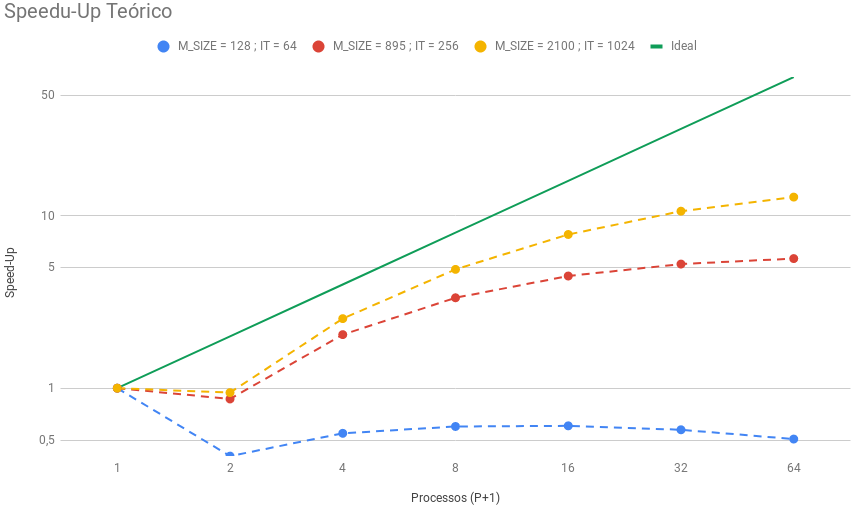
\includegraphics[width=15cm]{Pictures/TheoreticalGraph.png}
    \caption{Speed-up teórico}
\end{figure}

\begin{figure}[H]
    \centering
    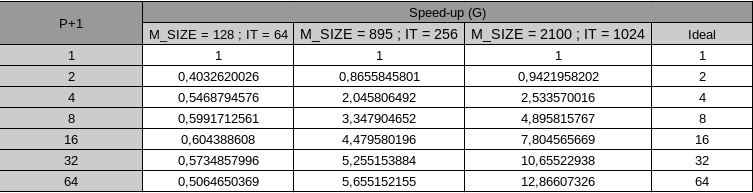
\includegraphics[width=15cm]{Pictures/TheoreticalTbl.png}
    \caption{Speed-up teórico}
\end{figure}

\section{Percentagem de Tempo de Comunicação}
\begin{figure}[H]
    \centering
    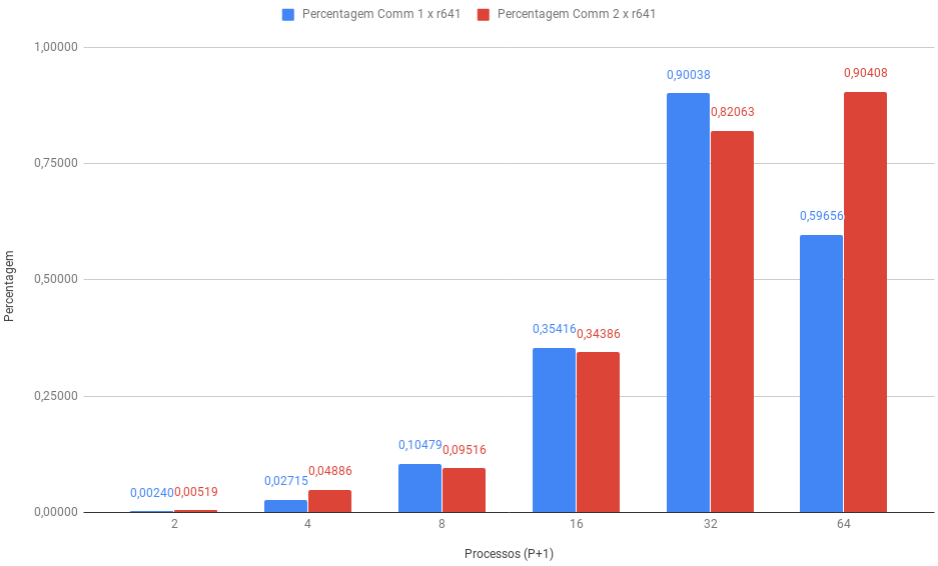
\includegraphics[width=18cm]{Pictures/histogramaPerc.png}
    \caption{Histograma das medianas das várias medianas de Tempo de Comunicação}
    \label{comm_time_perc}
\end{figure}

\section{Speed-up MPI Experimental}
\label{mpi_speedup_graph}
\begin{figure}[H]
    \centering
    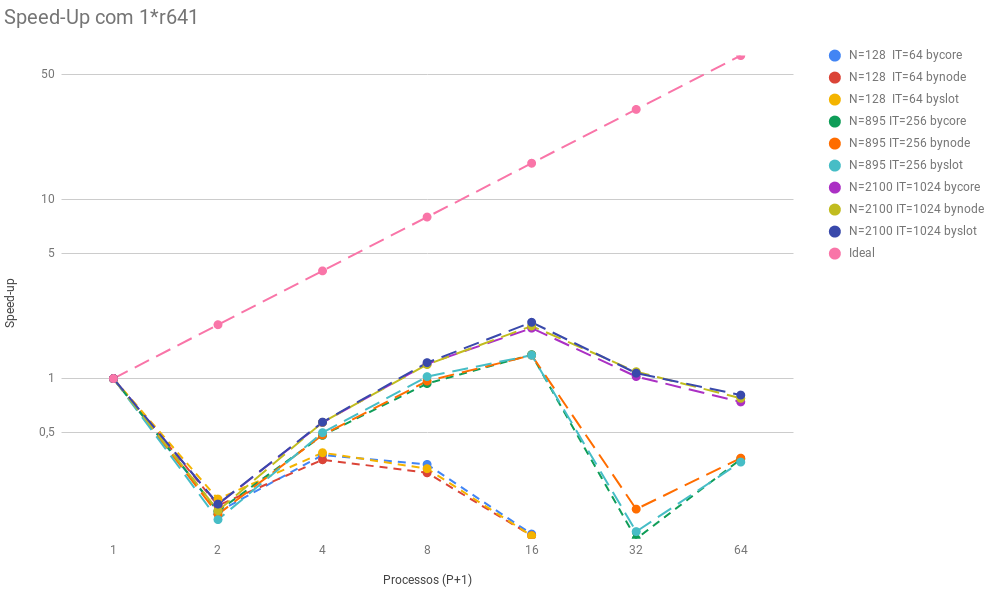
\includegraphics[width=16cm]{Pictures/ExperimentalGraph1.png}
    \caption{Speed-up experimental MPI com 1 nodo}
\end{figure}

\begin{figure}[H]
    \centering
    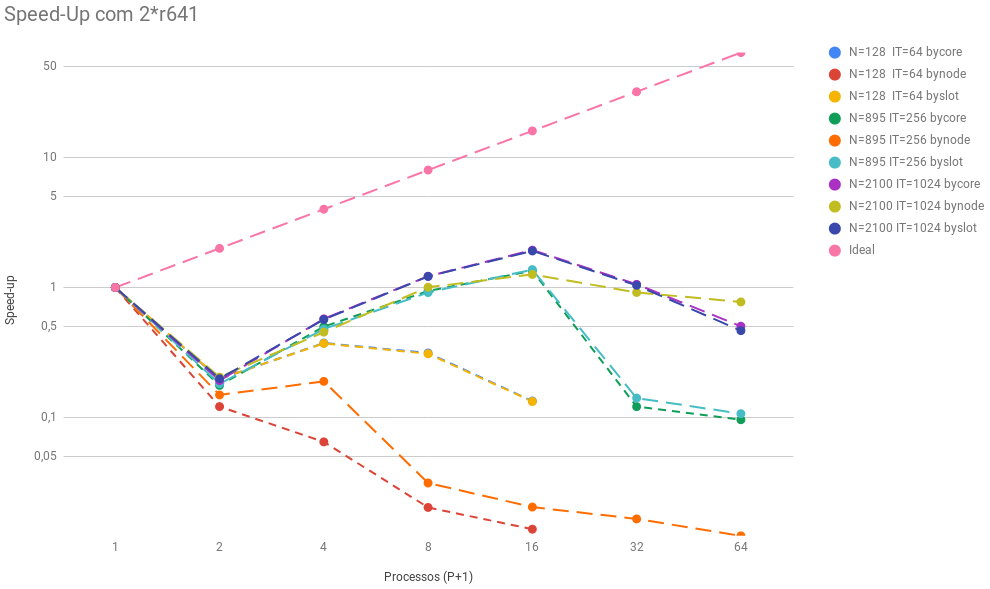
\includegraphics[width=16cm]{Pictures/ExperimentalGraph2.png}
    \caption{Speed-up experimental MPI com 2 nodos}
\end{figure}

\label{speedup_tbl}
\begin{figure}[H]
    \centering
    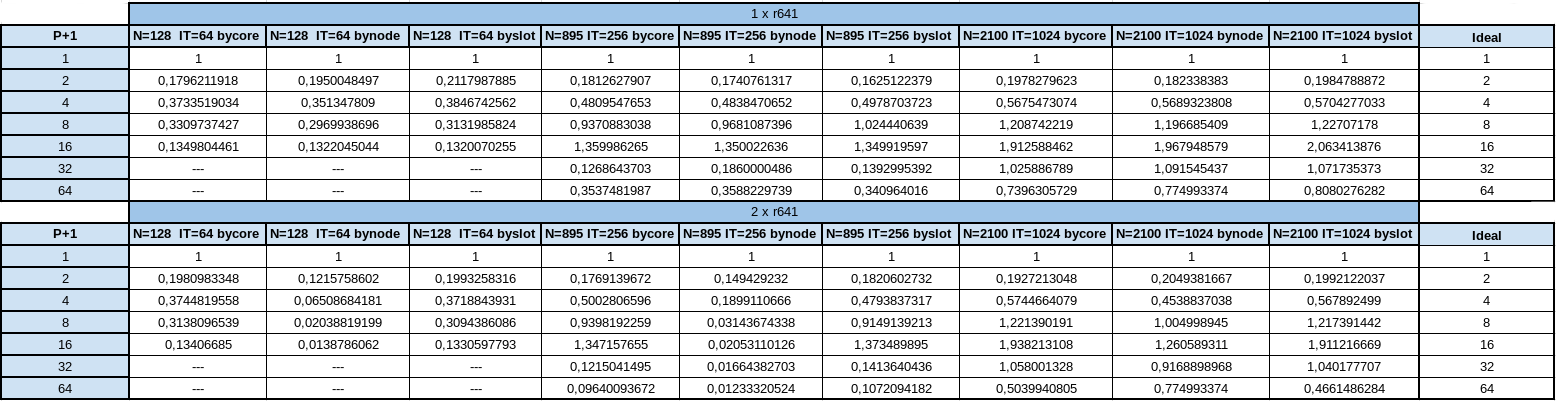
\includegraphics[width=19cm]{Pictures/ExperimentalTable.png}
    \caption{Speed-up MPI Experimental}
\end{figure}

\section{Speed-up OpenMP Experimental}
\label{mp_speedup_graph}
\begin{figure}[H]
    \centering
    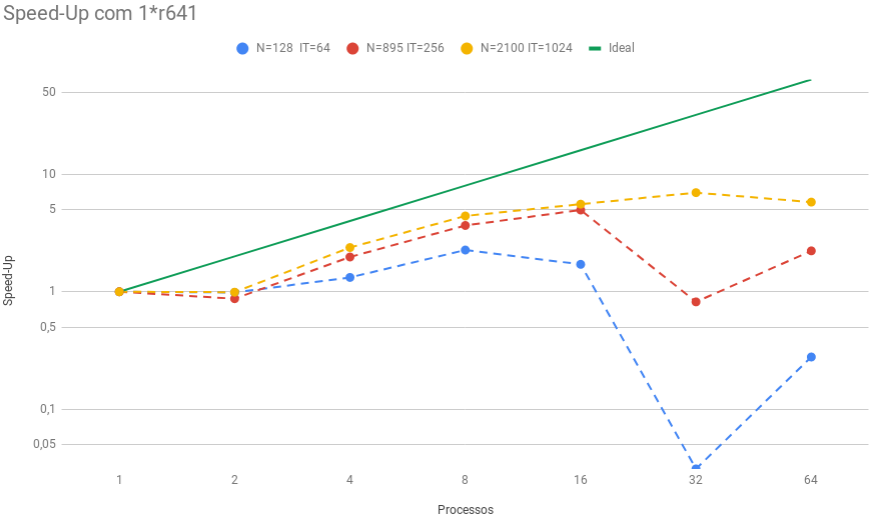
\includegraphics[width=16cm]{Pictures/OpenMP1.png}
    \caption{Speed-up OpenMP Experimental com 1 nodo r641}
\end{figure}

\begin{figure}[H]
    \centering
    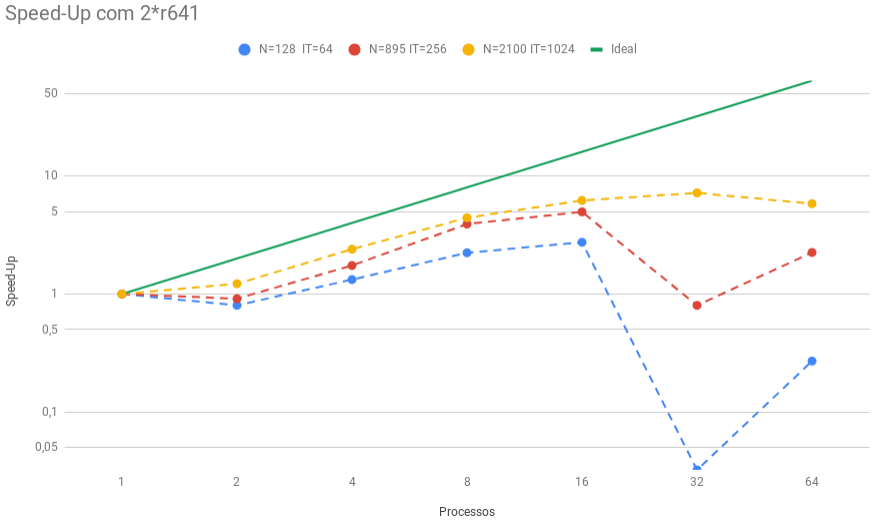
\includegraphics[width=16cm]{Pictures/OpenMP2.png}
    \caption{Speed-up OpenMP Experimental com 2 nodos r641}
\end{figure}

\begin{figure}[H]
    \centering
    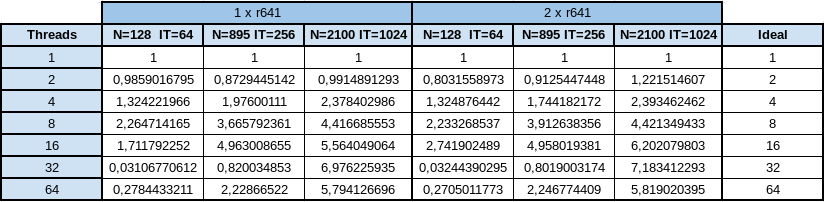
\includegraphics[width=18cm]{Pictures/OpenMPTable.png}
    \caption{Speed-up OpenMP Experimental}
\end{figure}

\section{Fluxo de dados}
\label{data_flux}
\begin{figure}[H]
    \centering
    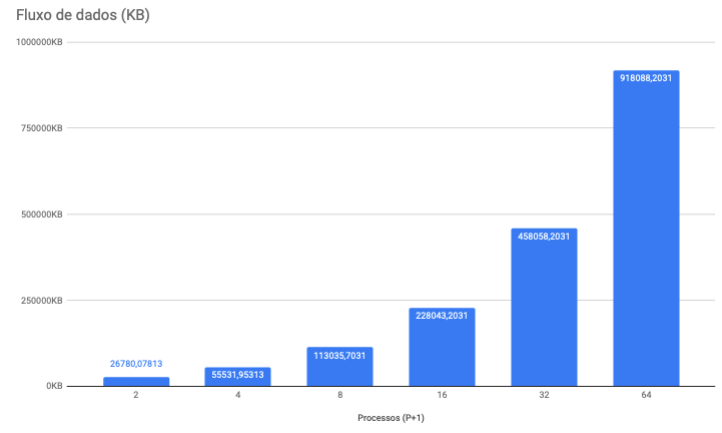
\includegraphics[width=15cm]{Pictures/DataFlux.png}
    \caption{Fluxo de dados em função do número de processos para N=895 e IT=256}
\end{figure}

\subsection{Fluxo de dados em função do número de processos (P) - Equação}
$$Kb=8*(2*M\_SIZE*M + 8*M\_SIZE*P + IT*2*4*M\_SIZE*(P-1)) $$

$$Kb=8*(2*895*887 + 8*895*P + 256*2*4*895*(P-1)) $$

\section{Contexto de experimentação}

\label{lab_config}
\begin{tabular}{|c|c|c|c|}
\hline
\textbf{Ordem(N) e Iterações(IT)} & \textbf{Nro. de processos} & \textbf{Mapeamento de processos} & \textbf{Nro. de nodos} r641 \\
\hline
N=128 IT=64              & 2, 4, 8, 16          & \texttt{--map-by} core, node, slot & 1, 2               \\
\hline
N=895 IT=256             & 2, 4, 8, 16, 32, 64  & \texttt{--map-by} core, node, slot & 1, 2               \\
\hline
N=2100 IT=1024           & 2, 4, 8, 16, 32, 64  & \texttt{--map-by} core, node, slot & 1, 2               \\
\hline
\end{tabular}

\end{appendices}

\end{document}
